\documentclass[compress]{beamer}

\mode<presentation>
{
  \usetheme{Madrid}       % or try default, Darmstadt, Warsaw, ...
  \usecolortheme{default} % or try albatross, beaver, crane, ...
  \usefonttheme[onlymath]{serif}    % or try default, structurebold, ...
  \setbeamertemplate{navigation symbols}{}
  \setbeamertemplate{caption}[numbered]
  \setbeamertemplate{headline}[default]
  \setbeamertemplate{blocks}[rounded][shadow=true]
  \useoutertheme[subsection=false]{miniframes}
} 

\usepackage[utf8]{inputenc}

\usepackage[square,sort,comma,numbers]{natbib}
\usepackage{graphicx}
\usepackage{amsmath,amsthm,amssymb}
\usepackage{mathtools}
\usepackage{multicol}
\usepackage{url}
\usepackage{todonotes}
\usepackage{lipsum}

\AtBeginSection[]{\subsection{}}

\DeclarePairedDelimiter{\abs}{\lvert}{\rvert}
\DeclarePairedDelimiter{\norm}{\lVert}{\rVert}

\let\vec\mathbf
\newcommand*{\C}{%
  \mathbb{C}%
}
\newcommand*{\R}{%
  \mathbb{R}%
}
\newcommand*{\Z}{%
  \mathbb{Z}%
}

\title[Graph Kernels]{Graph Kernels and Support Vector Machines for Pattern Recognition}
\author[Léo Andéol]{\textbf{Léo Andéol}\thanks{leo.andeol@gmail.com}\\ \footnotesize Supervised by: Prof. Hichem Sahbi}
\institute[Sorbonne Uni.]{Master DAC - Sorbonne Université}
\date{May 2019}

\begin{document}

\begin{frame}
  \titlepage
\end{frame}

\section{Introduction}
\begin{frame}{Summary}
  \tableofcontents[currentsection]
\end{frame}
\begin{frame}{Motivation}
\begin{multicols}{2}
	\begin{itemize}
		\item A lot of data can be represented as graphs such as proteins or social networks
		\item Being able to compare them would be useful (classification, clustering)
	\end{itemize}
	\begin{figure}
		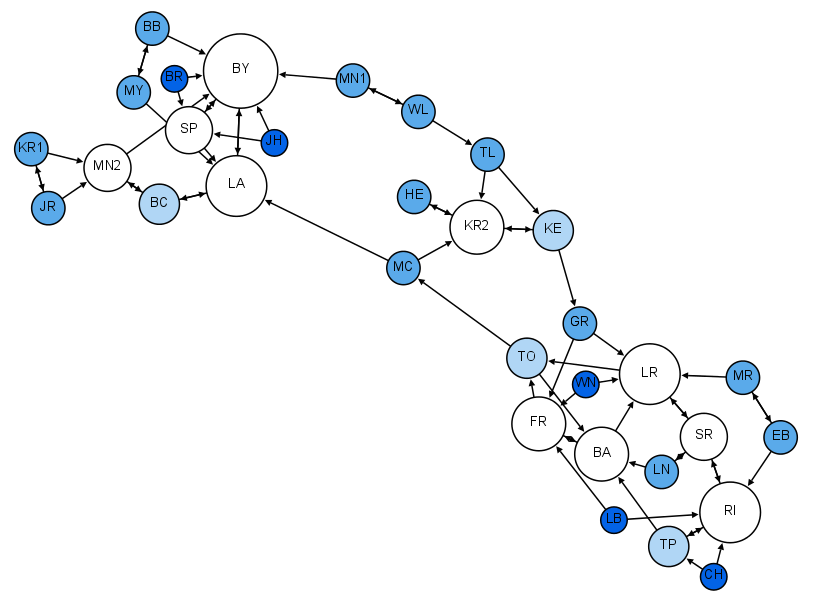
\includegraphics[height=.3\textheight]{data/sociogram.png}\par
		\caption{\footnotesize Moreno's sociogram (Source : Wikipedia)}
	\end{figure}
\end{multicols}

\begin{figure}
	\centering
	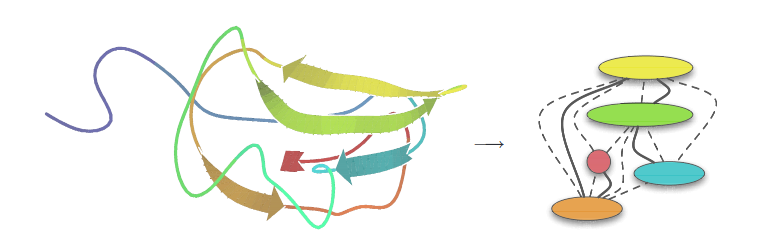
\includegraphics[height=.15\textheight, width=\linewidth]{data/ecoli.png}
\caption{A fragment of a protein transformed into a graph\cite{vishwanathan_graph_2010}}
\end{figure}

\end{frame}

\begin{frame}{Current Methods}
\begin{block}{Support Vector Machine}
SVMs are models used in classification introduced about 25 years ago. They have several advantages
\begin{itemize}
	\item Great accuracy
	\item Great capacity of generalization
	\item Allows the use of kernels in its dual form
\end{itemize}
\end{block}

\begin{block}{Kernels}
	The kernel trick can replace the dot product while implicitly projecting data to a feature space and combine very well with the SVMs
\begin{itemize}
	\item Computes data projection faster implicitly (ex. RBF kernel)
	\item Improve the accuracy of SVM by making linear separation easier
\end{itemize}
\end{block}
\end{frame}

\begin{frame}{Objective}
\begin{itemize}
	\item These methods are adapted to \textbf{vector data}
	\item Graphs and their adjacency matrices aren't and vectorizing implies a loss of information
	\item New types of kernels were discovered
	\item However, the complexity is a big problem, these kernels have to be accelerated
\end{itemize}
\begin{figure}
	\begin{multicols}{2}
		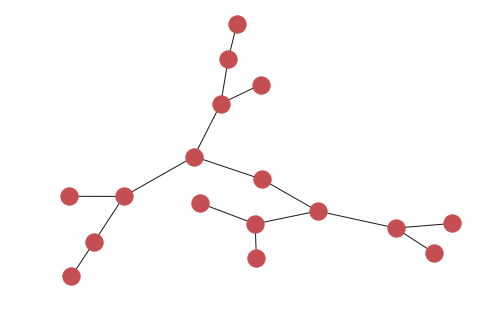
\includegraphics[width=\linewidth]{data/graphs/big_graph_no_label.png}
		$\begin{pmatrix}
		0 & 1 & 0 & 0 & 1 & 0 & 0 & 0 \\ 
		0 & 0 & 0 & 0 & 0 & 0 & 1 & 0 \\
		0 & 0 & 0 & 0 & 0 & 0 & 0 & 0 \\
		0 & 0 & 1 & 0 & 0 & 0 & 1 & 0 \\
		0 & 0 & 0 & 0 & 0 & 0 & 0 & 0 \\
		1 & 1 & 1 & 0 & 0 & 0 & 0 & 0 \\
		0 & 0 & 0 & 0 & 0 & 0 & 0 & 0 \\
		0 & 0 & 0 & 0 & 0 & 0 & 1 & 0 \\
		\end{pmatrix}$
	\end{multicols}
\caption{A tree graph and an adjacency matrix}
\end{figure}
\end{frame}


\section{Methodology}
\begin{frame}{Summary}
  \tableofcontents[currentsection]
\end{frame}
\begin{frame}{Background : graphs}
\begin{definition}
	A graph\cite{bondy1976graph} is a type of mathematical structure that represents connections between objects. It is more precisely an ordered pair $G=(V,E)$ of two sets: vertices $V$ (or nodes) and edges $E$ that connect two vertices together.
	\begin{equation*}
	E \subseteq \{(u,v) : (u,v) \in V^2\}
	\end{equation*}
\end{definition}
\begin{block}{Properties}
	\begin{multicols}{2}
		\begin{itemize}
			\item Undirected
			\item Labeled or not
			\item Degree
			\item Path and Cycle
		\end{itemize}
		\begin{itemize}
			\item Connected
			\item Tree
			\item Subgraph
			\item Line Graph
		\end{itemize}
	\end{multicols}
\end{block}
\end{frame}
\begin{frame}{Background : Support Vector Machines}
	\begin{block}{Classification}
		Classification is the problem of finding the best function $f :  \R^d \longrightarrow \{0..k\}$ among a set of functions $F$ while minimizing a risk function $R$
		\begin{equation*}
		f\star = \mbox{argmin}_f R(f)
		\end{equation*}
		where $k$ is the number of classes of the problem and $d$ the number of features of data 
	\end{block}
	\begin{block}{Support Vector Machines}
		\begin{equation*}
			\gamma_i = \frac{y_{i}(\vec{x}_{i} \cdot \vec{w} + w_{0})}{\norm{\vec{w}}}
		\end{equation*}
		\begin{equation*}
			\min \frac{1}{2}\norm{\vec{w}}^{2} \quad
			\textup{s.t.}\quad y_{i}(\vec{x}_{i} \cdot \vec{w} + w_{0}) \geq 1 \quad \forall i \in \{1..n\}
		\end{equation*}
	\end{block}
\end{frame}
\begin{frame}{Background : kernels}
	\begin{definition}
		In its dual form, the SVM problem only requires a dot product between the observations' vectors. 
		\begin{equation*}
		\text{max} \sum\limits_{i=1}^{n} \alpha_i - \frac{1}{2} \sum\limits_{j=1}^{n}\sum\limits_{i=1}^{n}\alpha_{i}\alpha_{j}y_{i}y_{j}\vec{x_{i}}^{\top}\vec{x_{j}}
		\end{equation*}
		This means the vectors can be mapped to higher dimensions with a function $\phi$. Moreover, even the dot product itself can be replaced by a function $\kappa$ without explicitly specifying the map $\phi$ as long as the function is positive semi definite.
		\begin{equation*}
		\kappa(\vec{x_{i}},\vec{x_{j}})={e}^{-\frac{\norm{\vec{x_{i}}-\vec{x_{j}}}^{2}}{2\sigma^{2}}}
		\end{equation*}
		\centering
		An example of kernel : the RBF kernel
	\end{definition}
\end{frame}
\begin{frame}{Graph Kernels}
    \begin{definition}
    	Graph Kernels are a type of R-convolution kernels\cite{haussler99convolution} applied to graphs, which are kernels that are based on decompositions of complex objects and comparisons of those decompositions.
    \end{definition}
	\begin{itemize}
		\item Random walks
		\item Graphlets
		\item Shortest paths, subtree
	\end{itemize}
\end{frame}
\begin{frame}{Graphlets}
rajouter info sur quels sont les graphlet
    \begin{definition}
   		Let $G$ and $G_2$ be two graphs, $\vec{f}_G$ and $\vec{f}_{G_2}$ the frequency vectors of respectively $G$ and $G_2$, then the kernel $\kappa$ is defined as
   		\begin{equation*}
   		\kappa(G,G_{2})=\vec{f}_{G}^{\top}\vec{f}_{G_2}
   		\end{equation*}
    \end{definition}
	\begin{itemize}
		\item Complexity of computing $\vec{f}_G$ is $O(n^k)$
		\item Sampling is required	
	\end{itemize}
\end{frame}
\begin{frame}{Random Walks}
\begin{block}{Random Walks}
	A random walk is a path obtained from a chosen vertex, randomly picking an edge to follow iteratively, until the trail reaches a certain length.
	Comparing common random walks between graphs is an acceptable metric.
\end{block}
\begin{block}{Product graph}
It has been shown\cite{imrich2000product} that computing random walks on two separate graphs is equivalent to computing it on the product graph of the two. The product graph is computed using the Kronecker (or tensor) product $\otimes$
$O(pn^6)$ complexity
\end{block}
\begin{figure}
\begin{multicols}{3}
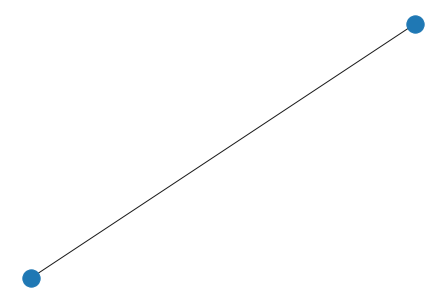
\includegraphics[width=1.5cm]{data/prod_graph/g1.png}\par
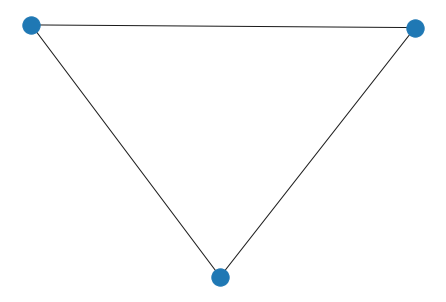
\includegraphics[width=1.5cm]{data/prod_graph/g2.png}\par
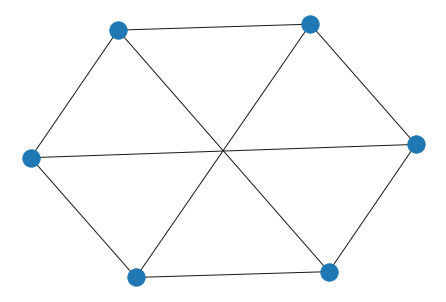
\includegraphics[width=1.5cm]{data/prod_graph/gx.png}\par
\end{multicols}
\caption{A graph $G_1$, a graph $G_2$ and the product graph $G_1 \otimes G_2$}
\end{figure}
\end{frame}
\begin{frame}{Random Walk}
	\begin{block}{Product graph}
		\begin{multicols}{2}
			\begin{itemize}
				\item $W_{\times}=A_1\otimes A_2$
				\item 
				$W_{\times}=\sum\limits_{l=1}^{d} A_1^{(l)} \otimes A_2^{(l)}$\\
			\end{itemize}
		\end{multicols}
	\end{block}
	\begin{block}{Kernel Definition}Let $p_{\times}$ and $q_{\times}$ be respectively the start and end probability of each node, and let $W_{\times}$ be the adjacency matrix of the product graph of $G$ and $G'$, and finally $\mu(k)$ be a convergent function of $k$.
		\begin{equation*}
		\kappa(G,G') = \sum\limits_{k=0}^{\infty}\mu(k)q_{\times}^{\top}W_{\times}^{k}p_{\times}
		\end{equation*}
	\end{block}
\end{frame}
\begin{frame}{Acceleration methods}
\begin{block}{Inverse Kernel}
A special case where $\mu(k)=\lambda^k$ leads to the following kernel
	\begin{equation*}
	\kappa(G_1,G_2)=q_{\times}^{\top}(I-\lambda W_\times)^{-1}p_{\times}
	\end{equation*}
\end{block}
\begin{itemize}
	\item $O(n^6)$ complexity
	\item Some methods will try to accelerate it
\end{itemize}
\end{frame}
\begin{frame}{Sylvester Equation}
complexity
\begin{definition}
	Let $A$, $B$, and $C$ be matrices of compatible shapes, then the Sylvester equation is
	\begin{equation*}
	AX+XB=C
	\end{equation*}
	And the discrete-time Sylvester Equation is 
	\begin{equation*}
	AXB+C=X
	\end{equation*}
	Which can be generalized as
	\begin{equation*}
	\sum_{i=0}^{d}A_{i}XB_{i}+C=X
	\end{equation*}
\end{definition}
\end{frame}
\begin{frame}{Conjugate Gradient}
	\begin{block}{Idea}
		\begin{itemize}
			\item The idea is to make new gradient orthogonal to the former
			\item Convergence guaranteed in $\abs{V}$ steps to solve the following problem
		\end{itemize}
		\begin{equation}
		(I-\lambda W_{\times})x=p_{\times}
		\end{equation}
	\end{block}
	\begin{figure}[!htb]
		\centering
		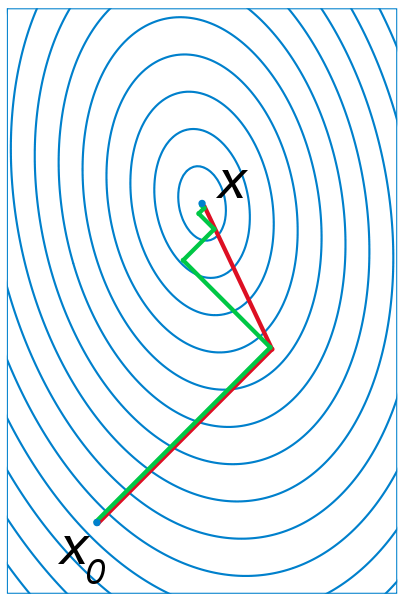
\includegraphics[height=0.3\textheight]{data/sota/conj_grad.png}
		\caption{Conjugate gradient (red) compared to Gradient Descent (green)}
		\label{fig:conj_grad}
	\end{figure} 
\end{frame}
\begin{frame}{Fixed Point Iterations}
\begin{block}{Definition}
Fixed point iterations is a method of computing a fixed point of a function by applying repeatedly the following equation until $\norm{x_{n+1}-x_{n}}<\epsilon$ where $\epsilon$ is the acceptable level of error.
\begin{equation*}
x_{n+1} = f(x_n)
\end{equation*}
Since this method requires the computation of $W_\times$, the kernel value can be computed for any type of labeling. For unlabeled graphs, the complexity is $O(kn^3)$ and $O(kdn^3)$ for labeled graphs, where $d$ is the number of labels and $k$ the number of iterations which can be estimated by
\begin{equation*}
k=O\left(\frac{\ln \epsilon}{\ln \lambda + \ln \abs{\xi}}\right)
\end{equation*}
\end{block}
\end{frame}
\begin{frame}{Spectral Decomposition}
\begin{block}{Definition}
	\begin{itemize}
		\item Eigendecomposition of the adjacency matrix
		\item Inverse becomes trivial to compute on diagonal matrix
	\end{itemize}
	\begin{equation*}
		 \kappa(G_1,G_2)=\sum\limits_{k=0}^{\infty}\mu(k)q_{\times}^{\top}(V_{\times}D_{\times}V_{\times}^{-1})^{k}p_{\times} = q_{\times}^{\top}V_{\times}\left(\sum\limits_{k=0}^{\infty}\mu(k)D_{\times}^{k}\right)V_{\times}^{-1}p_{\times}
	\end{equation*}
	However the following property is given from the Kronecker product
	\begin{equation*}
		A_1 \otimes A_2=(V_{1}D_{1}V_{1}^{-1})\otimes(V_{2}D_{2}V_{2}^{-1})=(V_1\otimes V_2)(D_1 \otimes D_2)(V_1 \otimes V_2)^{-1}
	\end{equation*}
	Taking advantage of that property
	\begin{equation}
	\kappa(G_1,G_2)=(q_{1}^{\top}V_{1}\otimes q_{2}^{\top}V_{2})(\sum\limits_{k=0}^{\infty}\mu(k)(D_{1}\otimes D_{2})^k)(V_{1}^{-1}p_{1}^{\top}\otimes V_{2}^{-1}p_{2}^{\top})
	\end{equation}
\end{block}
\end{frame}
\begin{frame}{Nearest Kronecker Product Approximation}
\begin{itemize}
	\item The idea is to approximate two matrices $S$ and $T$ such that $\norm{W_\times - A\otimes B}_F$ is minimized.
	\item Labeled-graph kernel computation can be turned into into an unlabeled one with some loss in accuracy, but gain in computation time.
	\item Computed in $O(dn^2)$ time 
	\item All methods such as Spectral Decomposition can then be applied
\end{itemize}
\end{frame}


\section{Experiments}
\begin{frame}{Summary}
  \tableofcontents[currentsection]
\end{frame}
\begin{frame}{Databases and metrics}
    \begin{block}{Synthetic Database}
    	A database of toy data was required to verify claims made in the studied article. A generator was written that can make graphs of "star", "tree" and "ring" types, of different sizes with different labels.
    \end{block}
	\pause
	\begin{block}{Real Databases}
		\begin{itemize}
			\item Proteins : 1113 proteins, 2 classes
			\item Enzymes : 600 enzymes, 6 classes
		\end{itemize}
	\end{block}
	\pause
	\begin{block}{Metrics}
		\begin{equation*}
		L(X,\vec{y})=\frac{1}{\abs{X}}\sum\limits_{i=1}^{\abs{X}}\left\{
		\begin{matrix}
		1 & \mbox{if } f(\vec{x}_i) \neq y_i \\
		0 & \mbox{otherwise}
		\end{matrix}
		\right.
		\end{equation*}
	\end{block}
\end{frame}
\begin{frame}{Implementation}
	%\setlength{\columnsep}{-2.1in}
	\begin{multicols}{2}
		\begin{itemize}
			\setlength\itemsep{4em}
			\item Sylvester Equation\\$A_{1}XA_{2}+C=X$
			\pause
			\item Conjugate Gradient\\$(I-\lambda W_{\times})x=p_{\times}$
			\pause
			\setlength\itemsep{4em}
			\item Fixed point\\$x_{t+1}=\lambda W_{\times}x_{t}+p_{\times}$
			\pause
			\item Spectral Decomposition\\$q_{\times}^{\top}P_{\times}(I-\lambda D_{\times})^{-1}P_{\times}^{-1}p_{\times}$
		\end{itemize}
	\end{multicols}
\end{frame}

\begin{frame}{Performance : Gram matrices}
\begin{figure}[!htb]
	\begin{multicols}{3}
		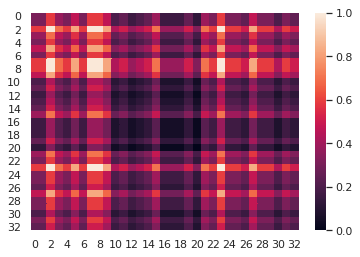
\includegraphics[width=\linewidth]{data/gram/gram3.png}\par
		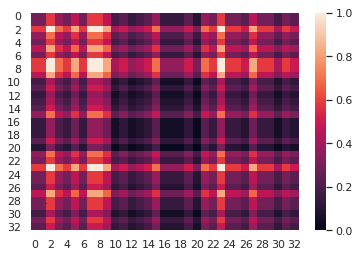
\includegraphics[width=\linewidth]{data/gram/gram4.png}\par
		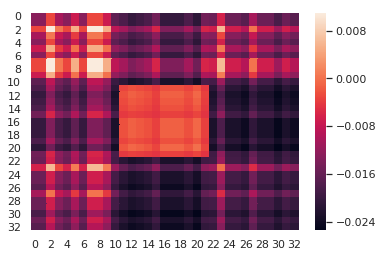
\includegraphics[width=\linewidth]{data/gram/gram5.png}\par
	\end{multicols}
	\caption{A gram matrix computed with the raw method, another with the fixed point method, and the difference between the two}
\end{figure}
\end{frame}

\begin{frame}{Performance : Gram matrices}
	\begin{table}[!htb]
		\begin{center}
			\begin{tabular}{|p{7mm}|p{9mm}|p{15mm}|p{15mm}|p{15mm}|p{15mm}|p{15mm}|p{15mm}|}
				\hline
				& Raw\newline kernel & Inverse\newline Kernel & Sylvester\newline Equation & Conjugate\newline Gradients & Fixed\newline points & Spectral\newline Decomp. \\
				\hline
				Raw. & 0 & 1.1e-4 & 9.8e-5 & 8.9e-5 & 1.0e-4 & 1.0e-04  \\
				\hline
				Inv. & - & 0 & 2.1e-5 & 7.9e-5 & 4.0e-6 & 6.8e-6 \\
				\hline
				Syl. & - & - & 0 & 8.0e-5 & 1.7e-5 & 1.4e-5  \\
				\hline
				Con. & - & - & - & 0 & 7.9e-5 & 7.9e-5  \\
				\hline
				Fix. & - & - & - & - & 0 & 2.8e-6 \\
				\hline
				Spe. & - & - & - & - & - & 0 \\
				\hline
			\end{tabular}
		\end{center}
		\caption {Mean standard deviation of matrix entries}
		\label{tab:frobenius_norm_diff} 
	\end{table}
\end{frame}

\begin{frame}{Performance : Label Use}
\begin{figure}[!htb]
	\begin{multicols}{2}
		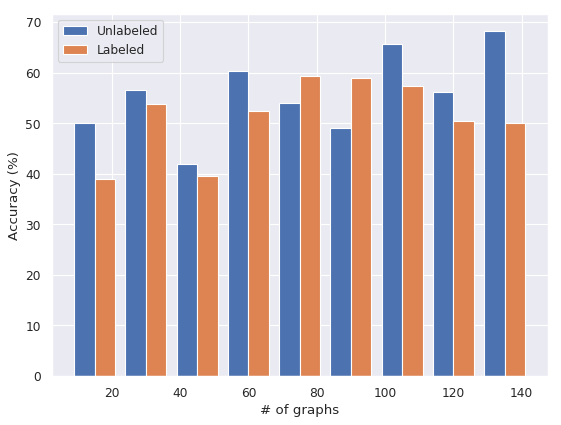
\includegraphics[width=\linewidth]{data/lab_nolab/acc.png}\par
		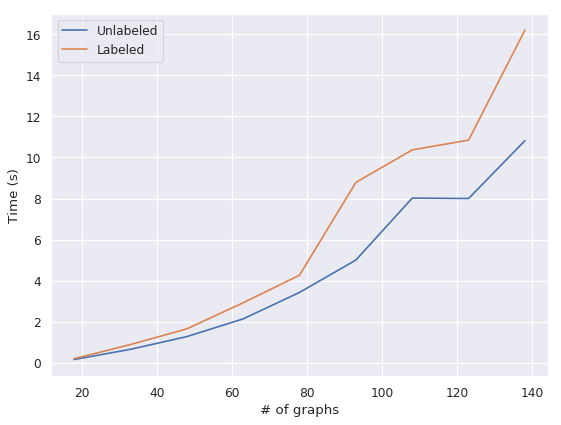
\includegraphics[width=\linewidth]{data/lab_nolab/time.png}\par
	\end{multicols}
	\caption {Accuracy and computation time of learning for unlabeled and labeled graphs}
\end{figure}
\end{frame}

\begin{frame}{Performance : Complexity}
\begin{figure}[!htb]
	\begin{multicols}{2}
		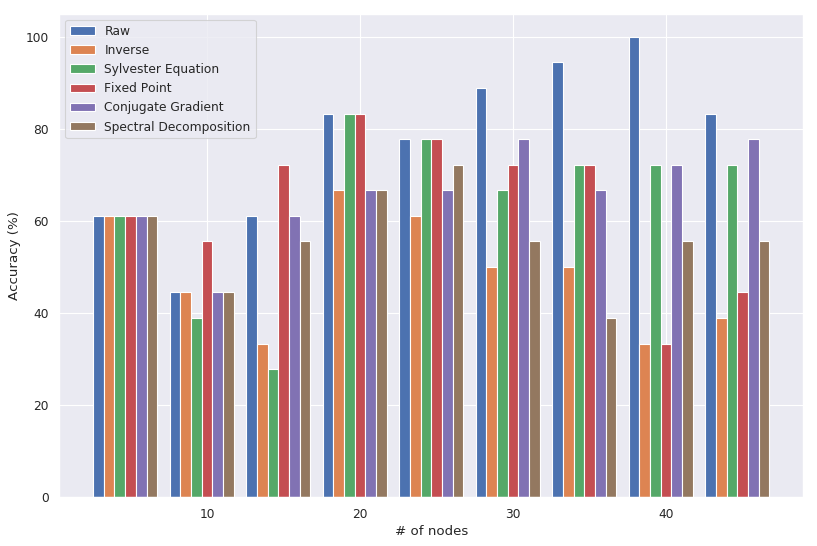
\includegraphics[width=\linewidth]{data/nb_nodes/acc.png}\par
		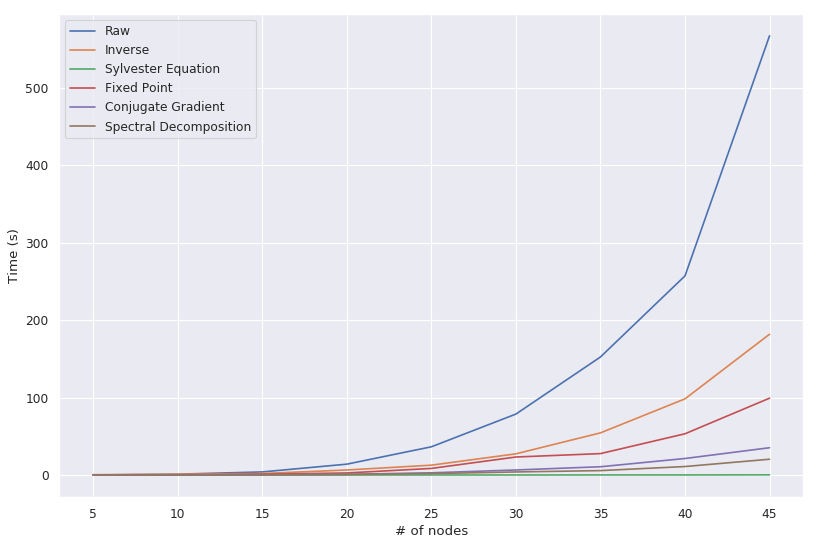
\includegraphics[width=\linewidth]{data/nb_nodes/time.png}\par
	\end{multicols}
	\caption{Accuracy and Computation time of different methods depending on the size of graphs}
\end{figure}
\end{frame}
\begin{frame}{Protein and Enzymes}

\end{frame}


\section{Conclusion}
\begin{frame}{Conclusion}
\begin{block}{Conclusion}
	\begin{itemize}
		\item Random walks : decent accuracy
		\item Several acceleration methods were introduced
		\item Performances are greatly improved
		\item conclusion on real data : todo
	\end{itemize}
\end{block}
\begin{block}{Future work}
	\begin{itemize}
		\item Generalized Sylvester Equation : algorithm and complexity
		\item Generalizing the Spectral Decomposition to labeled graphs
	\end{itemize}
\end{block}
\end{frame}

\renewcommand\bibsection{\subsection{\refname}}
\begin{frame}{References}
\nocite{bondy1976graph,borgwardt_protein_2005,imrich2000product,burges_tutorial_1998,vapnik_statistical_1998,nesterov_lectures_2018,shervashidze_efficient_2009}
\bibliographystyle{ieeetr}
\footnotesize
\bibliography{references}
\end{frame}

\appendix
\section[]{Appendix}
\begin{frame}[plain]{??}
??
\end{frame}


\end{document}